% Unofficial Yale Poster template.
% A fork of the UMich template https://www.overleaf.com/latex/templates/university-of-michigan-umich-poster-template/xpnqzzxwbjzc
% which is fork of the MSU template https://www.overleaf.com/latex/templates/an-unofficial-poster-template-for-michigan-state-university/wnymbgpxnnwd
% which is a fork of https://www.overleaf.com/latex/templates/an-unofficial-poster-template-for-new-york-university/krgqtqmzdqhg
% which is a fork of https://github.com/anishathalye/gemini
% also refer to https://github.com/k4rtik/uchicago-poster



\documentclass[final]{beamer}

% ====================
% Packages
% ====================

\usepackage[T1]{fontenc}
\usepackage[utf8]{luainputenc}
\usepackage{lmodern}
\usepackage[size=custom, width=121.92,height=91.44, scale=1.2]{beamerposter}
\usetheme{gemini}
\usecolortheme{msu}
\usepackage{graphicx}
\usepackage{booktabs}
\usepackage[numbers]{natbib}
\usepackage{tikz}
\usepackage{pgfplots}
\pgfplotsset{compat=1.14}
\usepackage{anyfontsize}
\usepackage{dsfont}
\usepackage{caption}
\usepackage{subcaption}
\usepackage{multirow}

% ====================
% Lengths
% ====================

% If you have N columns, choose \sepwidth and \colwidth such that
% (N+1)*\sepwidth + N*\colwidth = \paperwidth
\newlength{\sepwidth}
\newlength{\colwidth}
\setlength{\sepwidth}{0.025\paperwidth}
\setlength{\colwidth}{0.3\paperwidth}

\newcommand{\separatorcolumn}{\begin{column}{\sepwidth}\end{column}}

% ====================
% Title
% ====================

\title{Leveraging Alternative Data for Mixed Martial Arts Betting Markets}

\author{Eugene Han}

\institute[shortinst]{Yale University, Department of Statistics \& Data Science}

% ====================
% Footer (optional)
% ====================

\footercontent{
  \href{https://github.com/ehan03}{Github: ehan03} \hfill
 S\&DS Senior Thesis Poster Session \hfill
  \href{mailto:e.han@yale.edu}{Email: e.han@yale.edu}}
% (can be left out to remove footer)

% ====================
% Logo (optional)
% ====================

% use this to include logos on the left and/or right side of the header:
% Left: institution
 \logoright{
\includegraphics[height=8cm]{logos/logo.png}}
% Right: funding agencies and other affilations 
\logoleft{
\includegraphics[height=8cm]{logos/adobe-express-qr-code.png}}
% ====================
% Body
% ====================

\begin{document}



\begin{frame}[t]
\begin{columns}[t]
\separatorcolumn

\begin{column}{\colwidth}
  \vspace{-30pt}
  \begin{block}{Introduction}

    Beating the betting market for UFC fights is challenging due to outcome volatility and sparse data. Prior studies rely solely on the UFC Stats website, suffer from small backtesting samples, and have methodological flaws. Our work overcomes these limitations by curating a novel dataset from nontraditional sources and performing rigorous backtests, while also exploring new modeling and betting strategies inspired by robust optimization and conformal prediction.

  \end{block}

  \begin{block}{Dataset Curation}

    Data was scraped from 10 websites, cleaned, and standardized across sources, resulting in a 411 MB relational database with 58 tables, 6.9 million rows, and 64.7 million individual data points, $>$50$\times$ larger than UFC Stats alone (8 MB).
    \begin{itemize}
        \item \textbf{Striking/Grappling}: UFC Stats, ESPN
        \item \textbf{Betting Odds}: Best Fight Odds, FightOdds.io
        \item \textbf{Fight History/Rankings/Ratings}: Fight Matrix, Sherdog
        \item \textbf{Judge Scoring}: MMA Decisions
        \item \textbf{Miscellaneous}: Bet MMA, Tapology, Wikipedia
    \end{itemize}

  \end{block}

  \begin{block}{Feature Engineering}
    Features were created semi-systematically based on domain knowledge using only information strictly known \textbf{before} the start of a given event to eliminate leakage.
    
    \begin{itemize}
        \item \textbf{Event-Level}: Shared attributes across same-event fights (e.g., venue elevation)

        \item \textbf{Bout-Level}: Attributes of individual fights (e.g., weight class)

        \item \textbf{Fighter-Level}: Comparative measures based on fighters' attributes and past performance (e.g., difference in historical strikes landed per second)
    \end{itemize}

    % insert figures
    \begin{figure}
        \centering
        \captionsetup{justification=centering}
        \begin{subfigure}{.5\linewidth}
            \centering
            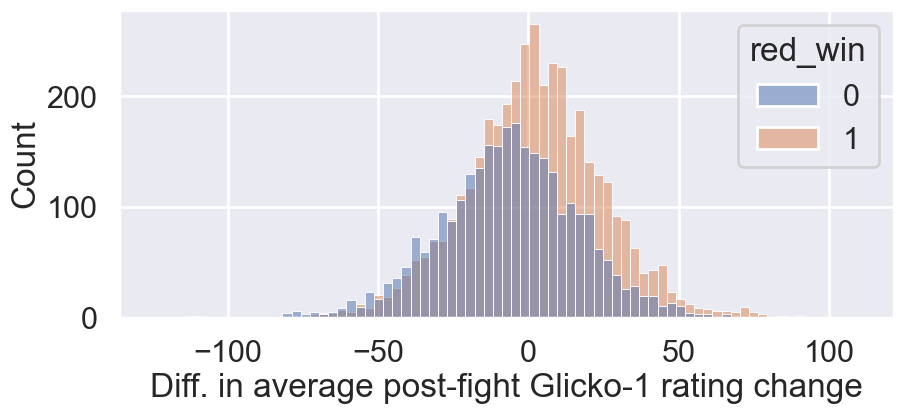
\includegraphics[width=\linewidth]{figures/glicko_1.png}
        \end{subfigure}
        \begin{subfigure}{.49\linewidth}
            \centering
            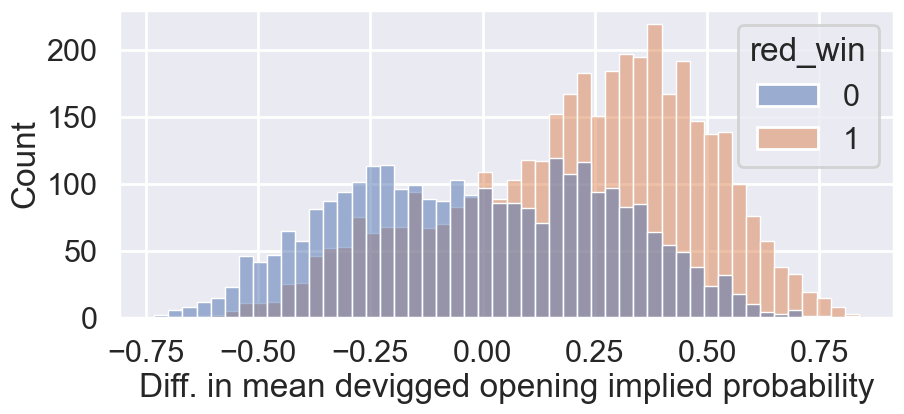
\includegraphics[width=\linewidth]{figures/opening_implied.png}
        \end{subfigure}\\
        \begin{subfigure}{.49\linewidth}
            \centering
            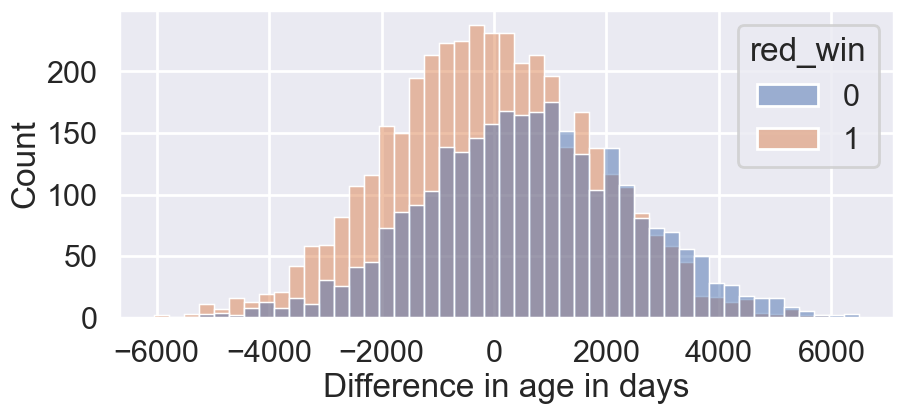
\includegraphics[width=\linewidth]{figures/age_days.png}
        \end{subfigure}
        \begin{subfigure}{.49\linewidth}
            \centering
            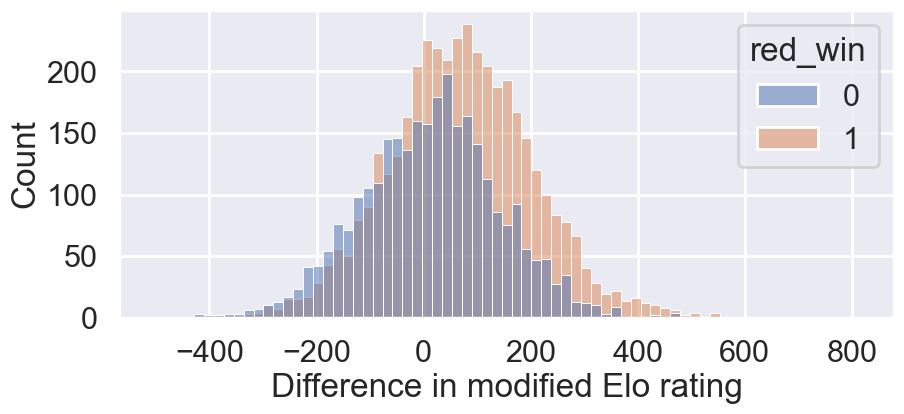
\includegraphics[width=\linewidth]{figures/elo_modified.png}
        \end{subfigure}
        \caption{Class distributions for selected examples of engineered features}
    \end{figure}

  \end{block}

  \begin{block}{Modeling Approach}
    Let $Y_i = \mathds{1}\{\text{red corner fighter wins fight } i\}$. \textbf{Goal}: Model $\mathbb{P}(Y_i = 1 \mid X_i)$.
    
    \begin{enumerate}
        \item \textbf{Odds Feature Ablation}: Inclusion/exclusion of opening odds-derived feature

        \item \textbf{Feature Selection}: Variance thresholding followed by top K selection via mutual information scores

        \item \textbf{Base Model}: Experimented with ridge logistic regression and gradient boosting

        \item \textbf{Calibration}: Inclusion/exclusion of using Venn-Abers predictors, which outputs an interval $(p_0, p_1)$ with validity guarantees such that
        $p_0 \leq \mathbb{P}(y = 1 \mid x) \leq p_1$
    \end{enumerate}

  \end{block}

\end{column}

\separatorcolumn

\begin{column}{\colwidth}
  \vspace{-30pt}
  \begin{block}{Betting Strategies}

    Suppose an event has $m$ fights. There exist $2m + 1$ bets and $2^m$ possible outcomes.

    \textbf{Simultaneous Kelly}: Find allocation $b$, to maximize expected log growth rate of wealth, $G_{\pi} (b) = \pi^T \log(R^Tb)$. For $m = 2$, construct $R$ and estimate $\pi$ as
    $$R = \begin{pmatrix}
    o_{r, 1} & o_{r, 1} & 0 & 0 \\
    0 & 0 & o_{b, 1} & o_{b, 1} \\
    o_{r, 2} & 0 & o_{r, 2} & 0 \\
    0 & o_{b, 2} & 0 & o_{b, 2} \\
    1 & 1 & 1 & 1
    \end{pmatrix}, \quad \hat{\pi} = \begin{pmatrix}
        \hat{p}_1 \hat{p}_2 \\
        \hat{p}_1 (1 - \hat{p}_2) \\
        (1 - \hat{p}_1) \hat{p}_2 \\
        (1 - \hat{p}_1) (1 - \hat{p}_2)
    \end{pmatrix}$$
    given odds $o_{r} = (o_{r,1}, \ldots, o_{r,m})$ , $o_b = (o_{b,1}, \ldots, o_{b,m})$ and $\hat{p}_j = \hat{\mathbb{P}}(Y_j = 1 \mid X_j)$.

    \textbf{Distributional Robust Kelly}: Maximize expected worst case log growth rate, $G_{\Pi}(b) = \inf_{\pi \in \Pi} G_{\pi} (b)$, over uncertainty set $\Pi = \{\pi \in \Delta_{2^m} \mid A \pi \leq d \}$ with
    $$A = \begin{pmatrix}
        - I_{2^m} \\
        I_{2^m}
    \end{pmatrix}, \quad d = \begin{pmatrix}
        -\hat{\pi}_{\text{lower}} \\
        \hat{\pi}_{\text{upper}}
    \end{pmatrix}$$
    where $\hat{\pi}_{\text{lower}}, \hat{\pi}_{\text{upper}}$ are defined like $\hat{\pi}$ using the $(p_0, p_1)$ outputs from Venn-Abers.

  \end{block}
  \vspace{-20pt}
  \begin{block}{Backtesting Setup}

    \begin{itemize}
        \item \textbf{Date Range}: 8-year period, 2017 to 2024 (3960 bouts, 331 events)

        \item \textbf{Training/Tuning}: Refit after every event, retune at end of each year

        \item \textbf{Bankroll Details}: Initial = \$1000, Kelly fraction $f \in \{0.10, 0.15, 0.25\}$

        \item \textbf{Benchmark}: Closing odds from Bovada Sportsbook

        \item \textbf{Significance Testing}: Monte Carlo simulations using closing odds with
        $$\text{p-value} = \frac{(\text{\# of simulations with profit}\geq\text{observed}) + 1}{(\text{total \# of simulations}) + 1}$$
        and adjusted using a Bonferroni correction
    \end{itemize}

  \end{block}
  \vspace{-20pt}
  \begin{block}{Model Results}

    \scriptsize
    \begin{table}[]
    \begin{tabular}{@{}lrr@{}}
    \toprule
    Model Pipeline                           & Log Loss          & Brier Score       \\ \midrule
    Logistic Regression                      & \textbf{0.608060} & 0.210443 \\
    Logistic Regression (No Odds)            & 0.629998          & 0.220371          \\
    Venn-Abers Logistic Regression           & 0.608881          & 0.210849          \\
    Venn-Abers Logistic Regression (No Odds) & 0.632596          & 0.221477          \\
    LightGBM                                 & 0.611128          & 0.211772          \\
    LightGBM (No Odds)                       & 0.631593          & 0.221174          \\
    Venn-Abers LightGBM                      & 0.611205          & 0.211956          \\
    Venn-Abers LightGBM (No Odds)            & 0.633977          & 0.222121          \\ \midrule
    \textit{Bovada Sportsbook}               & \textit{0.608142} & \textbf{\textit{0.210265}} \\ \bottomrule
    \end{tabular}
    \caption{Summary of model metrics over the backtest period, compared with closing odds}
    \end{table}
    \normalsize
    \vspace{-20pt}
    \begin{figure}
        \centering
        \captionsetup{justification=centering}
        \begin{subfigure}{.24\linewidth}
            \centering
            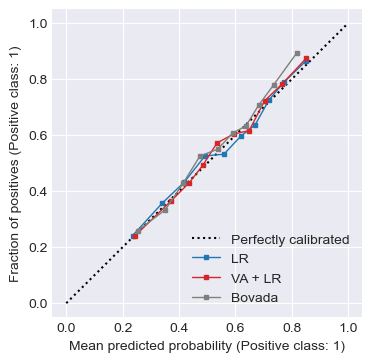
\includegraphics[width=\linewidth]{figures/lr_and_va.png}
        \end{subfigure}
        \begin{subfigure}{.24\linewidth}
            \centering
            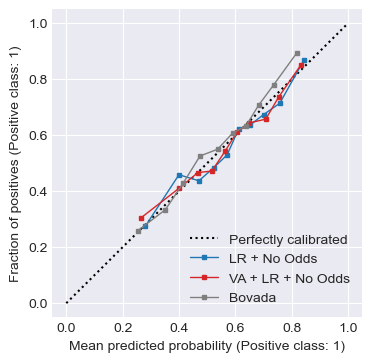
\includegraphics[width=\linewidth]{figures/lr_no_odds_and_va.png}
        \end{subfigure}
        \begin{subfigure}{.24\linewidth}
            \centering
            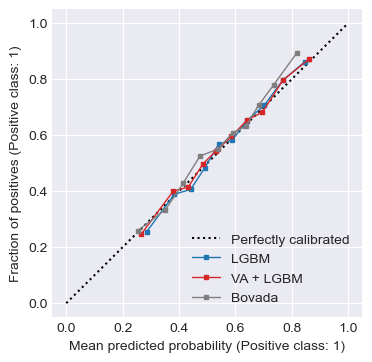
\includegraphics[width=\linewidth]{figures/lightgbm_and_va.png}
        \end{subfigure}
        \begin{subfigure}{.24\linewidth}
            \centering
            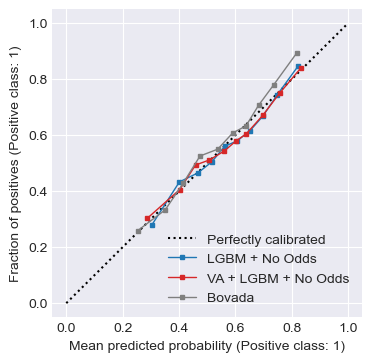
\includegraphics[width=\linewidth]{figures/lightgbm_no_odds_and_va.png}
        \end{subfigure}
        \caption{Calibration plots comparing model pipelines with and without Venn-Abers}
    \end{figure}
    \vspace{-20pt}
    \begin{figure}
        \centering
        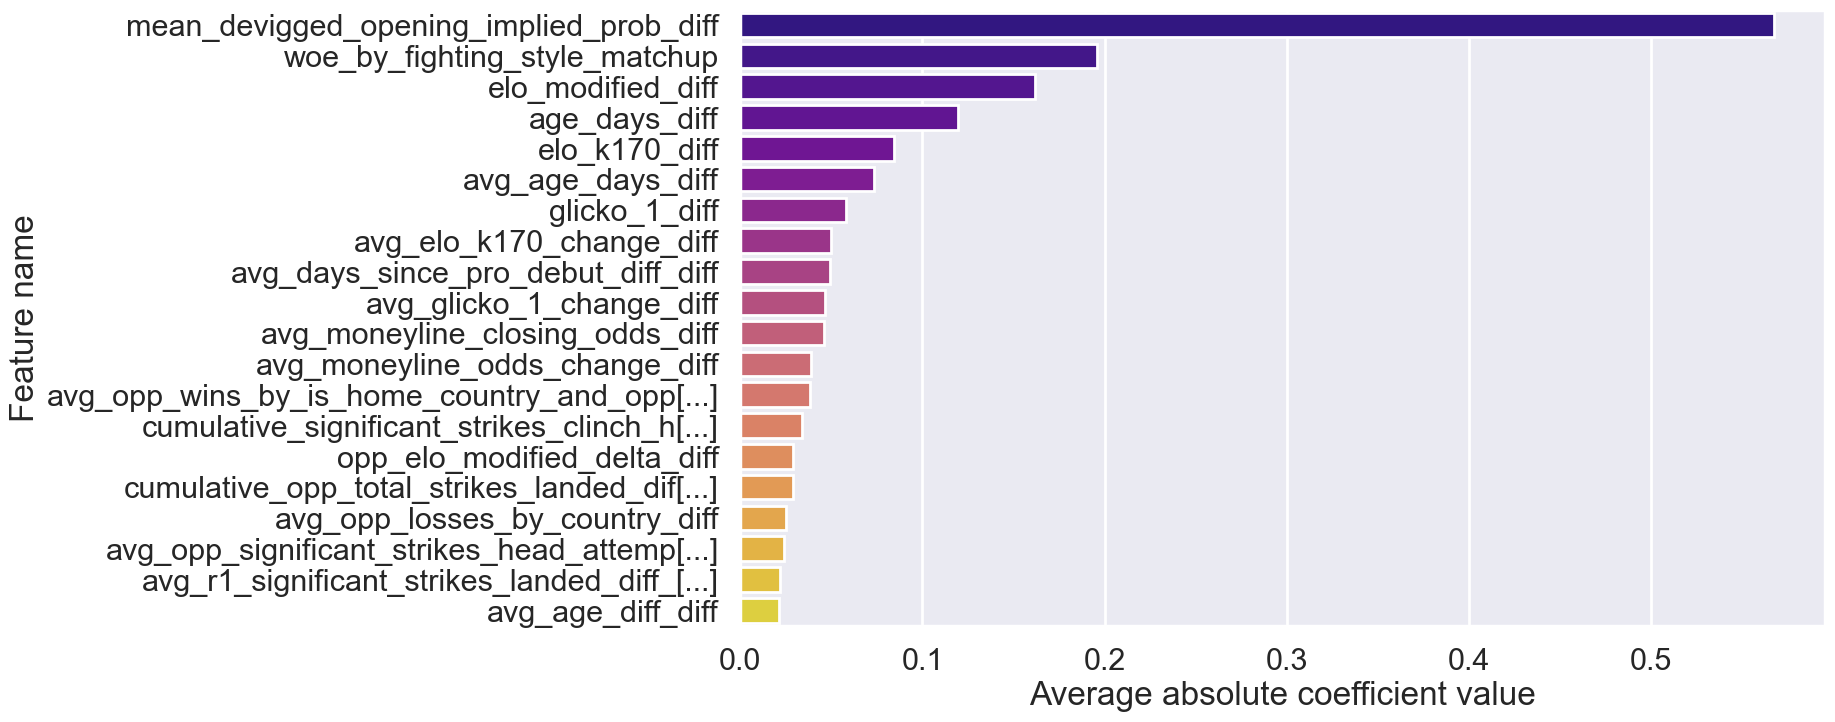
\includegraphics[width=0.6\linewidth]{figures/lr_feature_avg_abs_coef.png}
        \caption{Top 20 features by average absolute coefficient value in logistic regression model}
    \end{figure}
    

  \end{block}

\end{column}

\separatorcolumn

\begin{column}{\colwidth}
  \vspace{-30pt}
  \begin{block}{Betting Results}

    \scriptsize
    \begin{table}[]
    \begin{tabular}{@{}llrrrrrr@{}}
    \toprule
    Model Pipeline                                            & Betting Strategy                    & Fraction & Profit (\$) & Total Bets & Yield (\%) & MDD (\%) & Adj. p-value        \\ \midrule
    \multirow{3}{*}{Logistic Regression}                      & \multirow{3}{*}{Simultaneous} & 0.10     & 1318.98     & 1178       & 6.40       & -22.04            & \multirow{3}{*}{\textbf{0.0516}} \\
                                                              &                                     & 0.15     & 2159.40     & 1196       & 5.25       & -32.02            &                           \\
                                                              &                                     & 0.25     & \textbf{3763.63}     & 1201       & 3.47       & -50.46            &                           \\
    Logistic Regression (No Odds)                             & Simultaneous                  & 0.10     & -114.95       & 1810       & -0.53       & -40.19            & 0.9083                  \\
    \multirow{2}{*}{Venn-Abers Logistic Regression}           & Simultaneous                  & 0.10     & 430.80      & 1445       & 2.24       & -34.74            & 0.3528                  \\
                                                              & Distributional Robust        & 0.10     & 338.04      & 609        & \textbf{7.47}       & \textbf{-16.36}            & 0.3780                  \\
    \multirow{2}{*}{Venn-Abers Logistic Regression (No Odds)} & Simultaneous                 & 0.10     & -181.54      & 1865       & -0.78      & -45.45            & 1.0000                  \\
                                                              & Distributional Robust         & 0.10     & -260.40     & 1396       & -2.28      & -34.03            & 1.0000                  \\
    LightGBM                                                  & Simultaneous                 & 0.10     & 192.37      & 1610       & 0.89       & -49.20            & 0.5999                  \\
    LightGBM (No Odds)                                        & Simultaneous                 & 0.10     & -584.14     & 1906       & -3.29      & -68.99            & 1.0000                  \\
    \multirow{2}{*}{Venn-Abers LightGBM}                      & Simultaneous                  & 0.10     & 258.96      & 1540       & 1.21       & -46.78            & 0.5111                  \\
                                                              & Distributional Robust       & 0.10     & 130.44      & 881        & 1.93       & -30.03            & 1.0000                  \\
    \multirow{2}{*}{Venn-Abers LightGBM (No Odds)}            & Simultaneous                 & 0.10     & -551.64     & 1894       & -2.86      & -72.54            & 1.0000                  \\
                                                              & Distributional Robust        & 0.10     & -394.33     & 1380      & -2.57      & -62.51            & 1.0000                  \\ \bottomrule
    \end{tabular}
    \caption{Betting metrics by model pipeline and betting strategy combination}
    \end{table}
    \normalsize
    
    \begin{figure}
        \centering
        \captionsetup{justification=centering}
        \begin{subfigure}{.49\linewidth}
            \centering
            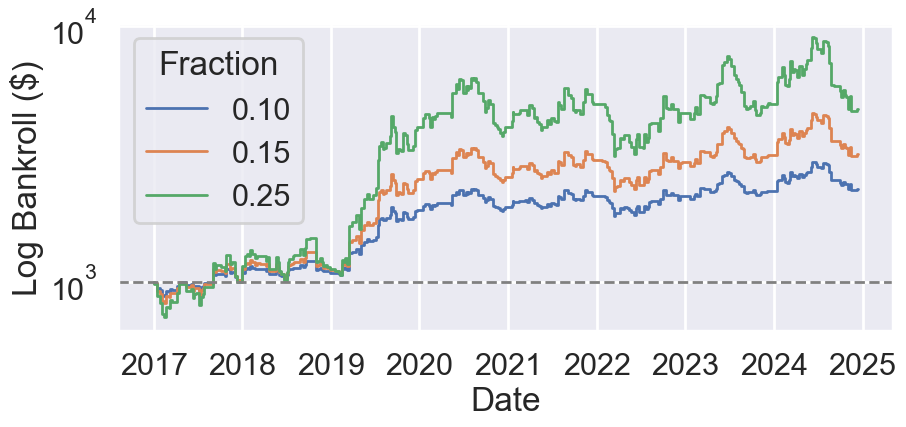
\includegraphics[width=\linewidth]{figures/lr_bankroll.png}
        \end{subfigure}
        \begin{subfigure}{.49\linewidth}
            \centering
            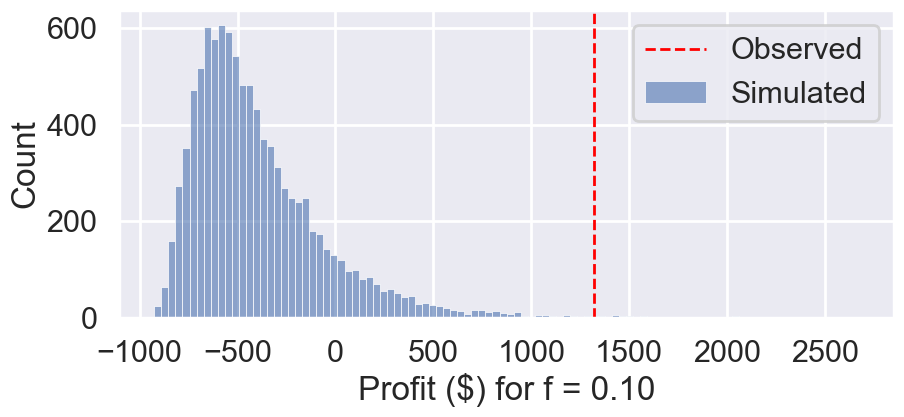
\includegraphics[width=\linewidth]{figures/lr_0.1_null_dist.png}
        \end{subfigure}
        \caption{Backtest performance for logistic regression and simultaneous Kelly}
    \end{figure}

  \end{block}
  \vspace{-6pt}
  \begin{block}{Case Study: Logistic Regression}
      \scriptsize
        \begin{table}[!htb]
        \centering
        \begin{tabular}{@{}lcc@{}}
        \toprule
                            & Log Loss & Brier Score \\ \midrule
        Logistic Regression & \textbf{0.611250} & \textbf{0.211724}    \\
        Bovada Sportsbook   & 0.616538 & 0.214093    \\ \bottomrule
        \end{tabular}
        \normalsize
        \caption{Model metrics with women's and debut fights removed}
        \end{table}

        \scriptsize
        \begin{table}[!htb]
        \centering
        \begin{tabular}{rrrrrr} 
        \toprule
        Fraction & Profit (\$) & Total Bets & Yield (\%) & MDD (\%) & Raw $p$-value            \\ 
        \midrule
        0.10     & 4758.95     & 964        & 15.99      & -20.56   & \multirow{3}{*}{0.0001}  \\
        0.15     & 11306.91    & 974        & 14.21      & -29.42   &                          \\
        0.25     & 43830.51    & 976        & 11.07      & -46.47   &                          \\
        \bottomrule
        \end{tabular}
        \normalsize
        \caption{Betting metrics with women's and debut fights removed}
        \end{table}
  
      \begin{figure}
        \centering
        \captionsetup{justification=centering}
        \begin{subfigure}{.49\linewidth}
            \centering
            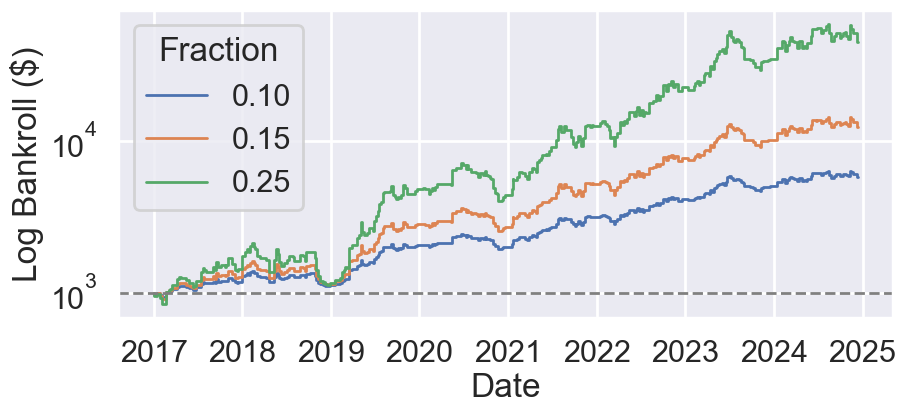
\includegraphics[width=\linewidth]{figures/lr_case_study_bankroll.png}
        \end{subfigure}
        \begin{subfigure}{.49\linewidth}
            \centering
            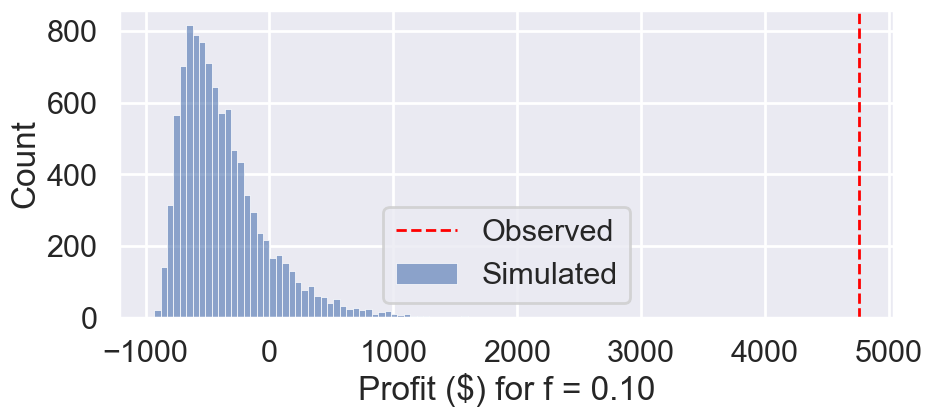
\includegraphics[width=\linewidth]{figures/lr_case_study_0.1_null_dist.png}
        \end{subfigure}
        \caption{Backtest performance with women's and debut fights removed}
    \end{figure}
  \end{block}
\vspace{-6pt}
  \begin{block}{Discussion and Future Work}
      \begin{itemize}
          \item Clear value-add from incorporating sources other than UFC Stats

          \item Betting performance looks promising but continued forward testing is required

          \item Untapped potential in database to improve methods or answer new questions
      \end{itemize}
  \end{block}
\vspace{-6pt}
  \begin{block}{References}

    \nocite{*}
    \scriptsize{\bibliographystyle{plainnat}\bibliography{poster}}

  \end{block}

\end{column}

\separatorcolumn
\end{columns}
\end{frame}

\end{document}
